\documentclass[simplex.tex]{subfiles}
% NO NEED TO INPUT PREAMBLES HERE
% packages are inherited; you can compile this on its own
\providecommand{\mb}[1]{\boldsymbol{#1}}
\providecommand{\mv}[1]{\vec{#1}}
\providecommand{\ve}[1]{\boldsymbol{#1}}
\newcommand{\bpsi}{\ve{\psi}}
\newcommand{\bv}{\mb{v}}
\newcommand{\bx}{\mb{x}}
\newcommand{\bA}{\mathbf{A}}
\newcommand{\bH}{\mathbf{H}}
\newcommand{\bX}{\mathbf{X}}
\newcommand{\bP}{\mathbf{P}}
\newcommand{\bB}{\mathbf{B}}
\newcommand{\bD}{\mathbf{D}}
\newcommand{\bS}{\mathbf{S}}
\newcommand{\bR}{\mathbf{R}}
\newcommand{\bJ}{\mathbf{J}}
\newcommand{\bLambda}{\mathbf{\Lambda}}
\begin{document}
\subsection{Discriminability}
We develop a measure of discriminability (or reliability).  It
is intuitive to understand and easy to implement.
Discriminability is defined to be the probability of within
subject distances being smaller than the cross subject
distances. If we let $x_{i,t}$ denote the t$^{\text{th}}$ trial of subject 
$i$ and $\Delta(,)$ be the metric, the (population) discriminability $D$
is: 
\[D:= P (\Delta(x_{i,t} , x_{i,t’}) \leq  \Delta(x_{i,t} , x_{i’,t’’})).\]
Previously, we search for the optimal processing pipeline which has the
maximal discriminability. 
\\
Currently, we are considering the discriminability from a different perspective. Specifically, we want to use the discriminability as an internal measure of the consistency in clustering. If we let $x_{i,t}$ denote the t$^{\text{th}}$ sample of cluster 
$i$ and $\Delta(,)$ be the metric, the discriminability $D$
is: $D:= P (\Delta(x_{i,t} , x_{i,t’}) \leq  \Delta(x_{i,t} , x_{i’,t’’}))$. Large discriminability implies the clusters are more consistent, that is we can better differentiate samples from different clusters. 
\\
We are also developing a clustering algorithm \ref{alg:dcl} which maximizes the discriminability. The algorithm will assign each sample $i$ a cluster identity $k_i$ such that the discriminability is maximized. The algorithm is similar to K-means, but we believe discriminability provides a more robust measure than within cluster distances which is maximized in K-means.


\subsubsection*{Discriminability Algorithms}

\begin{algorithm}               
	\caption{Cluster samples through maximizing discriminability.  }   
	\label{alg:dcl}                       
	\begin{algorithmic}                    
		\Require Samples $\{\bx_{i}\}$ and number of clusters $K$.
		\Ensure Cluster identity $\{k_{i}\}$. 
		\Function{DiscriminabilityClustering}{}
		\State Initialize $\{k_{i}\}$ randomly
		\While{ not convergent}
		\For{$i$} 
		\For{$j$ in $1:K$}
		\State Set $k_{i} = j$ 
		\State ComputeDiscriminability($\{\bx_{i}\}$,$\{k_{i}\}$)
		\EndFor
		\State Set $k_{i}$ to the cluster with maximum discriminability
		\EndFor 
		\EndWhile
		\State Output $\{k_{i}\}$ 
		\EndFunction
	\end{algorithmic}
\end{algorithm}


\begin{algorithm}               
	\caption{Compute discriminability estimate $\hat{D}$.  }   
	\label{alg:dhat}                       
	\begin{algorithmic}                    
		\Require Test-retest samples $\{\bx_{i,t}\}$.
		\Ensure Sample discriminability $\hat{D}$. 
		\Function{ComputeDiscriminability}{}
		\For{$i,t,i',t'$} \Comment{compute pairwise distances}
		\State $PD[i,t,i',t'] = \delta(\bx_{i,t},\bx_{i',t'})$
		\EndFor
		\State Dsum = 0;
		\State Count = 0;
		\For{$i = 1,...,n$} 
		\For{$t = 1,...,s$}
		\State $d =$ across subject distances to $\bx_{i,t}$
		\For{$t' = 1,...,s$ and $t' \neq t$}
		\State $\hat{D}_{i,t,t'} =\sum_j {\bf I}\{PD[i,t,i,t'] < d[j]\}/Length(d)$ \Comment{compare within and across distances}
		\State $Dsum = Dsum + \hat{D}_{i,t,t'}$
		\State $Count = Count + 1$
		\EndFor	
		\EndFor
		\EndFor
		\State $\hat{D} = Dsum / Count$ \Comment{Sample Discrminability}
		\EndFunction
	\end{algorithmic}
\end{algorithm}

\begin{algorithm}               
	\caption{The function returns a p-value for testing the null hypothesis that $D = 0.5$.  }   
	\label{alg:ost}                       
	\begin{algorithmic}                    
		\Require Test-retest samples $\{\bx_{i,t}\}$, the number of permutations $np$.
		\Ensure The p-value $p \in [0,1]$ for testing the hypothesis that $D = 0.5$. 
		\Function{OneSampleTest}{}
		\State $\hat{D}= ComputeDiscriminability(\{\bx_{i,t}\})$ \Comment{compute true sample discriminability}
		\For{$j = 1,...,np$} 
		\State $\{\bx^{(j)}_{i,t}\} = Permute(\{\bx_{i,t}\})$ \Comment{permute the subject labels}
		\State $d[j] = ComputeDiscriminability(\{\bx^{(j)}_{i,t}\})$ \Comment{compute discriminability of permuted samples}
		\EndFor
		\State $p = \sum_j {\bf I}\{\hat{D} < d[j]\} / np$ \Comment{compute p-value}
		\EndFunction
	\end{algorithmic}
\end{algorithm}

\begin{algorithm}               
	\caption{The function returns a p-value for testing the null hypothesis that $D(\bpsi_1)=D(\bpsi_2)$.  }   
	\label{alg:tst}                       
	\begin{algorithmic}                    
		\Require Raw data $\{f_\phi(\bv_i)\}$ , pipeline $\bpsi_1$, pipeline $\bpsi_2$, the number of bootstrapped samples $nb$.
		\Ensure The p-value $p \in [0,1]$ for testing the hypothesis that $D(\bpsi_1)=D(\bpsi_2)$. 
		\Function{TwoSampleTest}{}
		\State $\{^1\bx_{i,t}\}= g_{\bpsi_1}(\{f_\phi(\bv_i)\})$ 
		\State $\{^2\bx_{i,t}\}= g_{\bpsi_1}(\{f_\phi(\bv_i)\})$ \Comment{process the raw data with two pipelines}
		\State $\hat{D}(\bpsi_1)=ComputeDiscriminability(\{^1\bx_{i,t}\})$
		\State $\hat{D}(\bpsi_2)=ComputeDiscriminability(\{^1\bx_{i,t}\})$ \Comment{compute sample discriminability estimates}
		\For{$j = 1,...,nb$} 
		\For{$i = 1,...,n$} 
		\State $i_1, i_2 = Sample(n)$ \Comment{randomly select two subjects}
		\State $\lambda = SampleUniform$ 
		\For{t = 1,...,s}  
		\State $^1\bx^{(j)}_{i,t} =  ^1\bx_{i_1,t} \lambda +   ^1\bx_{i_2,t}(1-\lambda)$ \Comment{Linearly combine two observations}
		\EndFor
		\EndFor
		\State $\hat{D}^{(j)}(\bpsi_1)=ComputeDiscriminability(\{^1\bx^{(j)}_{i,t}\})$
		\State $\hat{D}^{(j)}(\bpsi_2)=ComputeDiscriminability(\{^2\bx^{(j)}_{i,t}\})$
		\EndFor
		\State $ind = 0$
		\For{$j = 1,...,nb$} \Comment{generate the null distribution}
		\For{$j' = i+1,...,nb$}
		\State $d[ind] =  \hat{D}^{(j)}(\bpsi_1)-\hat{D}^{(j')}(\bpsi_1)$ 
		\State $ind = ind + 1$
		\State $d[ind] =  \hat{D}^{(j)}(\bpsi_2)-\hat{D}^{(j')}(\bpsi_2)$
		\State $ind = ind + 1$
		\EndFor
		\EndFor
		\State $p = \sum_j {\bf I}\{\hat{D}(\bpsi_1)-\hat{D}(\bpsi_2) < d[j]\} / Length(d)$ \Comment{compute p-value}
		\EndFunction
	\end{algorithmic}
\end{algorithm}

\clearpage

\subsection{Joint Embedding}
We developed a method to jointly embed multiple graphs/networks. Previous spectral embedding techniques work on each graph separately. Our joint embedding approach generalizes Adjacency Spectral Embedding to multiple graphs. Specifically,  the joint embedding method identifies a linear subspace spanned by rank one symmetric matrices and projects adjacency matrices of graphs into this subspace. Given $m$ graphs $\{G_i \} _{i=1}^{m}$ with $\bA_i$ being the corresponding adjacency matrix, the $d$-dimensional joint embedding of graphs $\{G_i \} _{i=1}^{m}$ is given by
 \begin{equation*}
 	\begin{aligned}  
 	(\hat{\bH},\hat{\bD}_1,...,\hat{\bD}_m) =	& \underset{\bD_i,\|h_k\|=1}{\operatorname{argmin}} 
 		& & \sum\limits_{i=1}^{m} \| \bA_i- \bH \bD_i \bH^T \|  ^2 \\
 		& \text{ subject to} 
 		& &  \bD_i \text{ being diagonal.}
 	\end{aligned}
 \end{equation*}
Here, $h_k$ is the $k$th column of matrix $\bH$. The $\hat{\bH}$ are estimated latent positions for vertices, and the diagonal of $\hat{\bD}_i$ can be treat as the feature of graph $i$. We performed theoretical and numerical analysis of the joint embedding. The code and paper can be found \href{https://github.com/shangsiwang/Joint-Embedding}{here}.  

We study predicting individual composite creativity index (CCI) through brain connectomes obtained by Multimodal Magnetic Resonance Imaging. In total, $113$ healthy, young adult subjects were scanned and their CCI is assessed by independent judges using the Consensual Assessment Technique. First, we jointly embed brain graphs of all subjects. Figure \ref{fig:cci1} shows a typical graph and $\hat{h}_6 \hat{h}_6^T$ estimated by the joint embedding. Next, we construct a linear regression model by treating the diagonal of $\hat{\bD}_i$ as explanatory variables and CCI as the response variable. 

Overall, the regression model for predicting CCI is significant at level $0.05$ compared to the null model. We found CCI positively correlated to overall connectivity of the brain. Furthermore, we found CCI significantly negatively related to $\hat{h}_6 \hat{h}_6^T$. This implies that compared to within hemisphere connectivity across hemisphere connectivity has a larger positive impact on human creativity. 


%%%  FIGURE BLOCK
\begin{figure}[!h]
\begin{cframed}
\centering
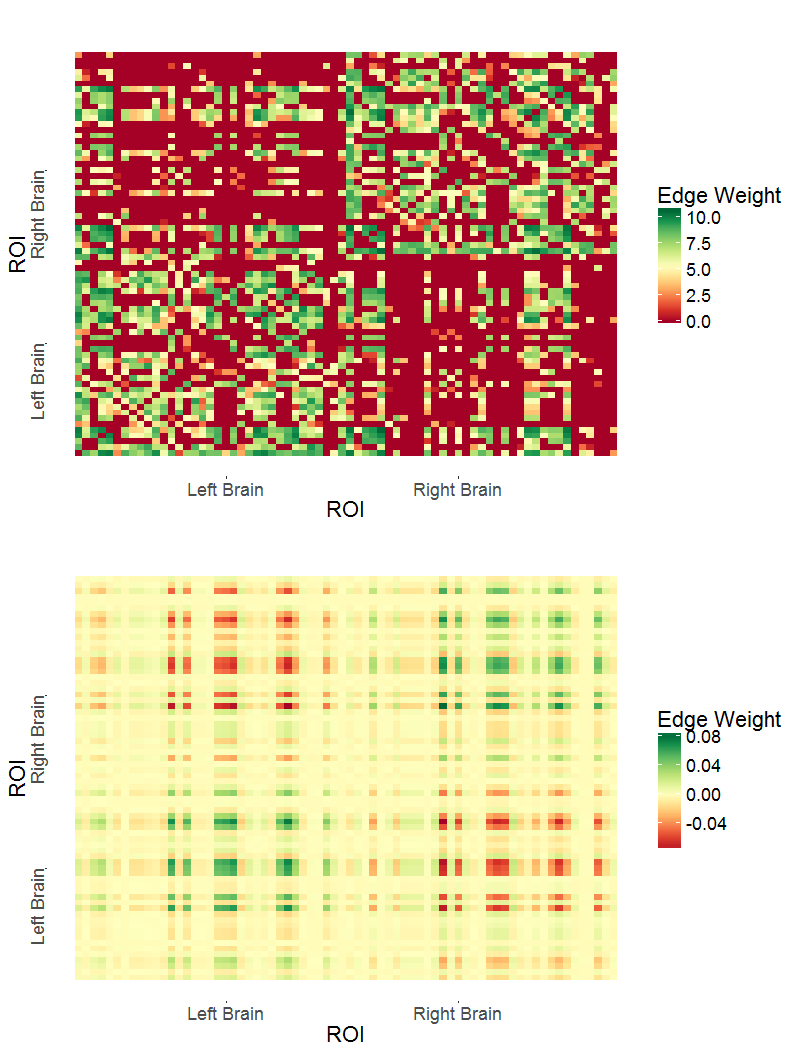
\includegraphics[scale=0.25, clip = true, trim = 0 7in 0 .5in]{../../figs/cci_data.png}
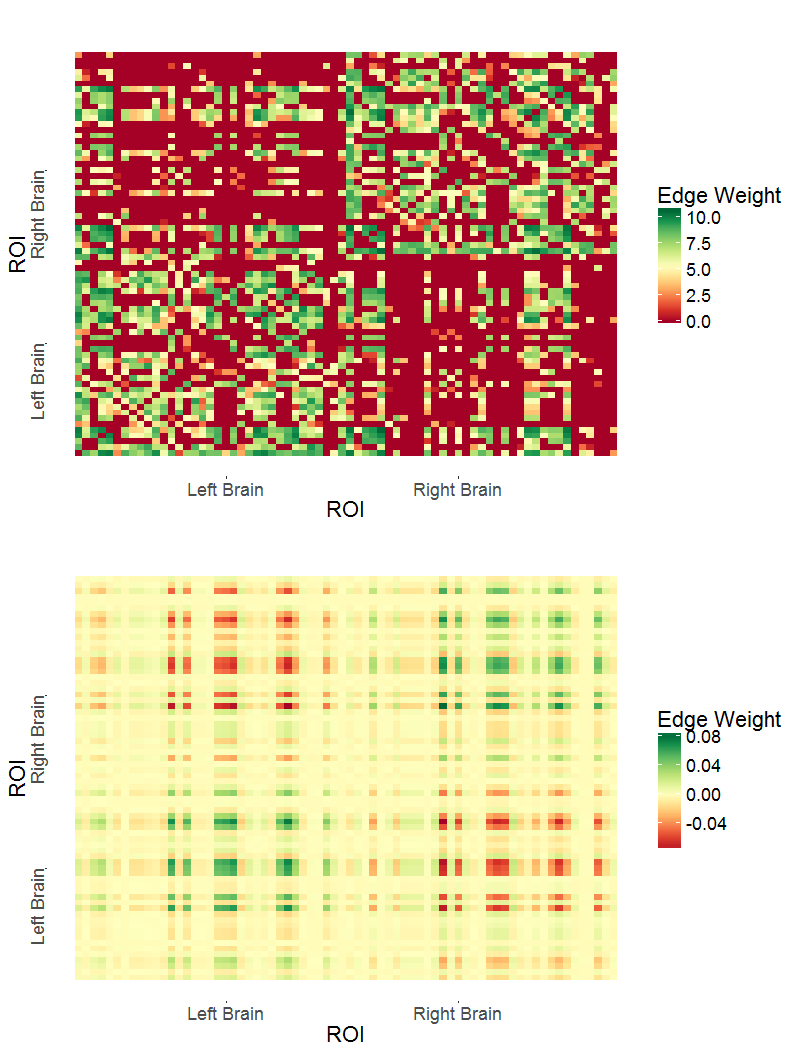
\includegraphics[scale=0.25, clip = true, trim = 0 -0.45in 0 8in]{../../figs/cci_data.png}
%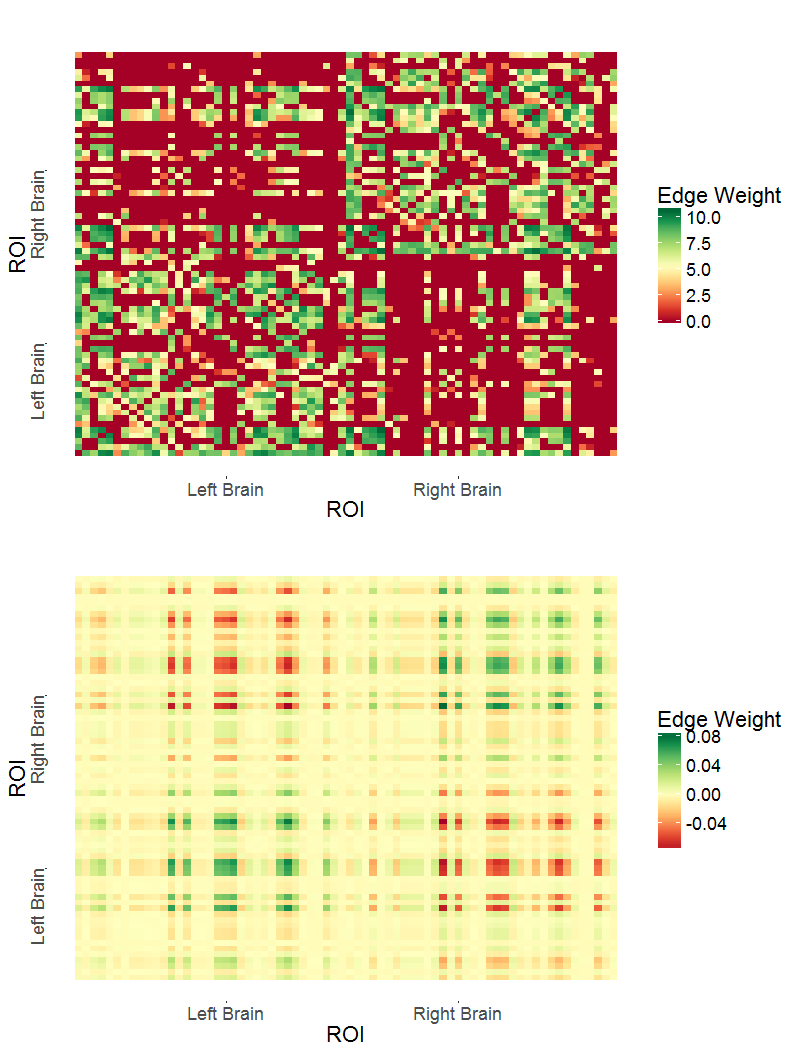
\includegraphics[scale=0.25]{../../figs/cci_data.png}
\caption{The left panel shows the graph derived from a typical subject.
  There is much more neural connectivity within each hemisphere. The
  right panel shows the rank one matrix $\hat{h}_6^T\hat{h}_6$, which
  has positive  connectivity within each hemisphere, but negative
  connectivity across hemispheres.}
\label{fig:cci1}
\end{cframed}
\end{figure}
%
\clearpage

\end{document}
